\SourceLeaf{339}

Ferner, bezeichnen wir z.\,B. den Winkel, welchen (I, II) mit der festen Axe bildet, mit [I, II],
so haben wir:
\[
\begin{array}{rl}
\text{[I, II]} & = [4,1] + [3,2] \\
\text{[II, III]} & = [2,1] + [4,3] \\
\text{[III, I]} & = [3,1] + [4,2].
\end{array}
\]
Folglich haben wir: Es ist der Winkel:
\[
\begin{array}{rl}
\text{II, I, III} & = [4,1] + [3,2] - [3,1] - [4,2] \\
\text{III, II, I} & = [2,1] + [4,3] - [4,1] - [3,2] \\
\text{I, III, II} & = [3,1] + [4,2] - [2,1] - [4,3].
\end{array}
\]

Wendet man also den Satz an, dass sich in einem Dreieck die Seiten verhalten, wie die Sinus der
gegenüberliegenden Winkel, so hat man für das ursprüngliche Viereck:
\[
\begin{aligned}
&\frac{\sin\{[4,1]+[3,2]-[3,1]-4,2]\}}{(2,1)(4,3)}\\
&=\frac{\sin\{[2,1]+[4,3]-[4,1]-[3,2]\}}{(3,1)(4,2)}\\
&=\frac{\sin\{[3,1]+[4,2]-[2,1]-[4,3]\}}{(4,1)(3,2)}.
\end{aligned}
\]

\Needspace{27\baselineskip}\begin{center}
[2.]
\end{center}

Unser Satz lässt sich ebenso einfach geometrisch beweisen, weshalb wir den letztern Beweis
gleichfalls hierher setzen, obgleich er eigentlich nicht in diesen Vortrag gehört.

Wir nehmen zuerst den Fall an, es läge der Punkt 4 innerhalb des Dreiecks 1, 2, 3. Zieht man dann
(4,1), (4,2), (4,3) und verlängert die Richtungen dieser Linien bis nach I, II, III, so dass man
habe:

\begin{center}\resizebox{12.8cm}{!}{%
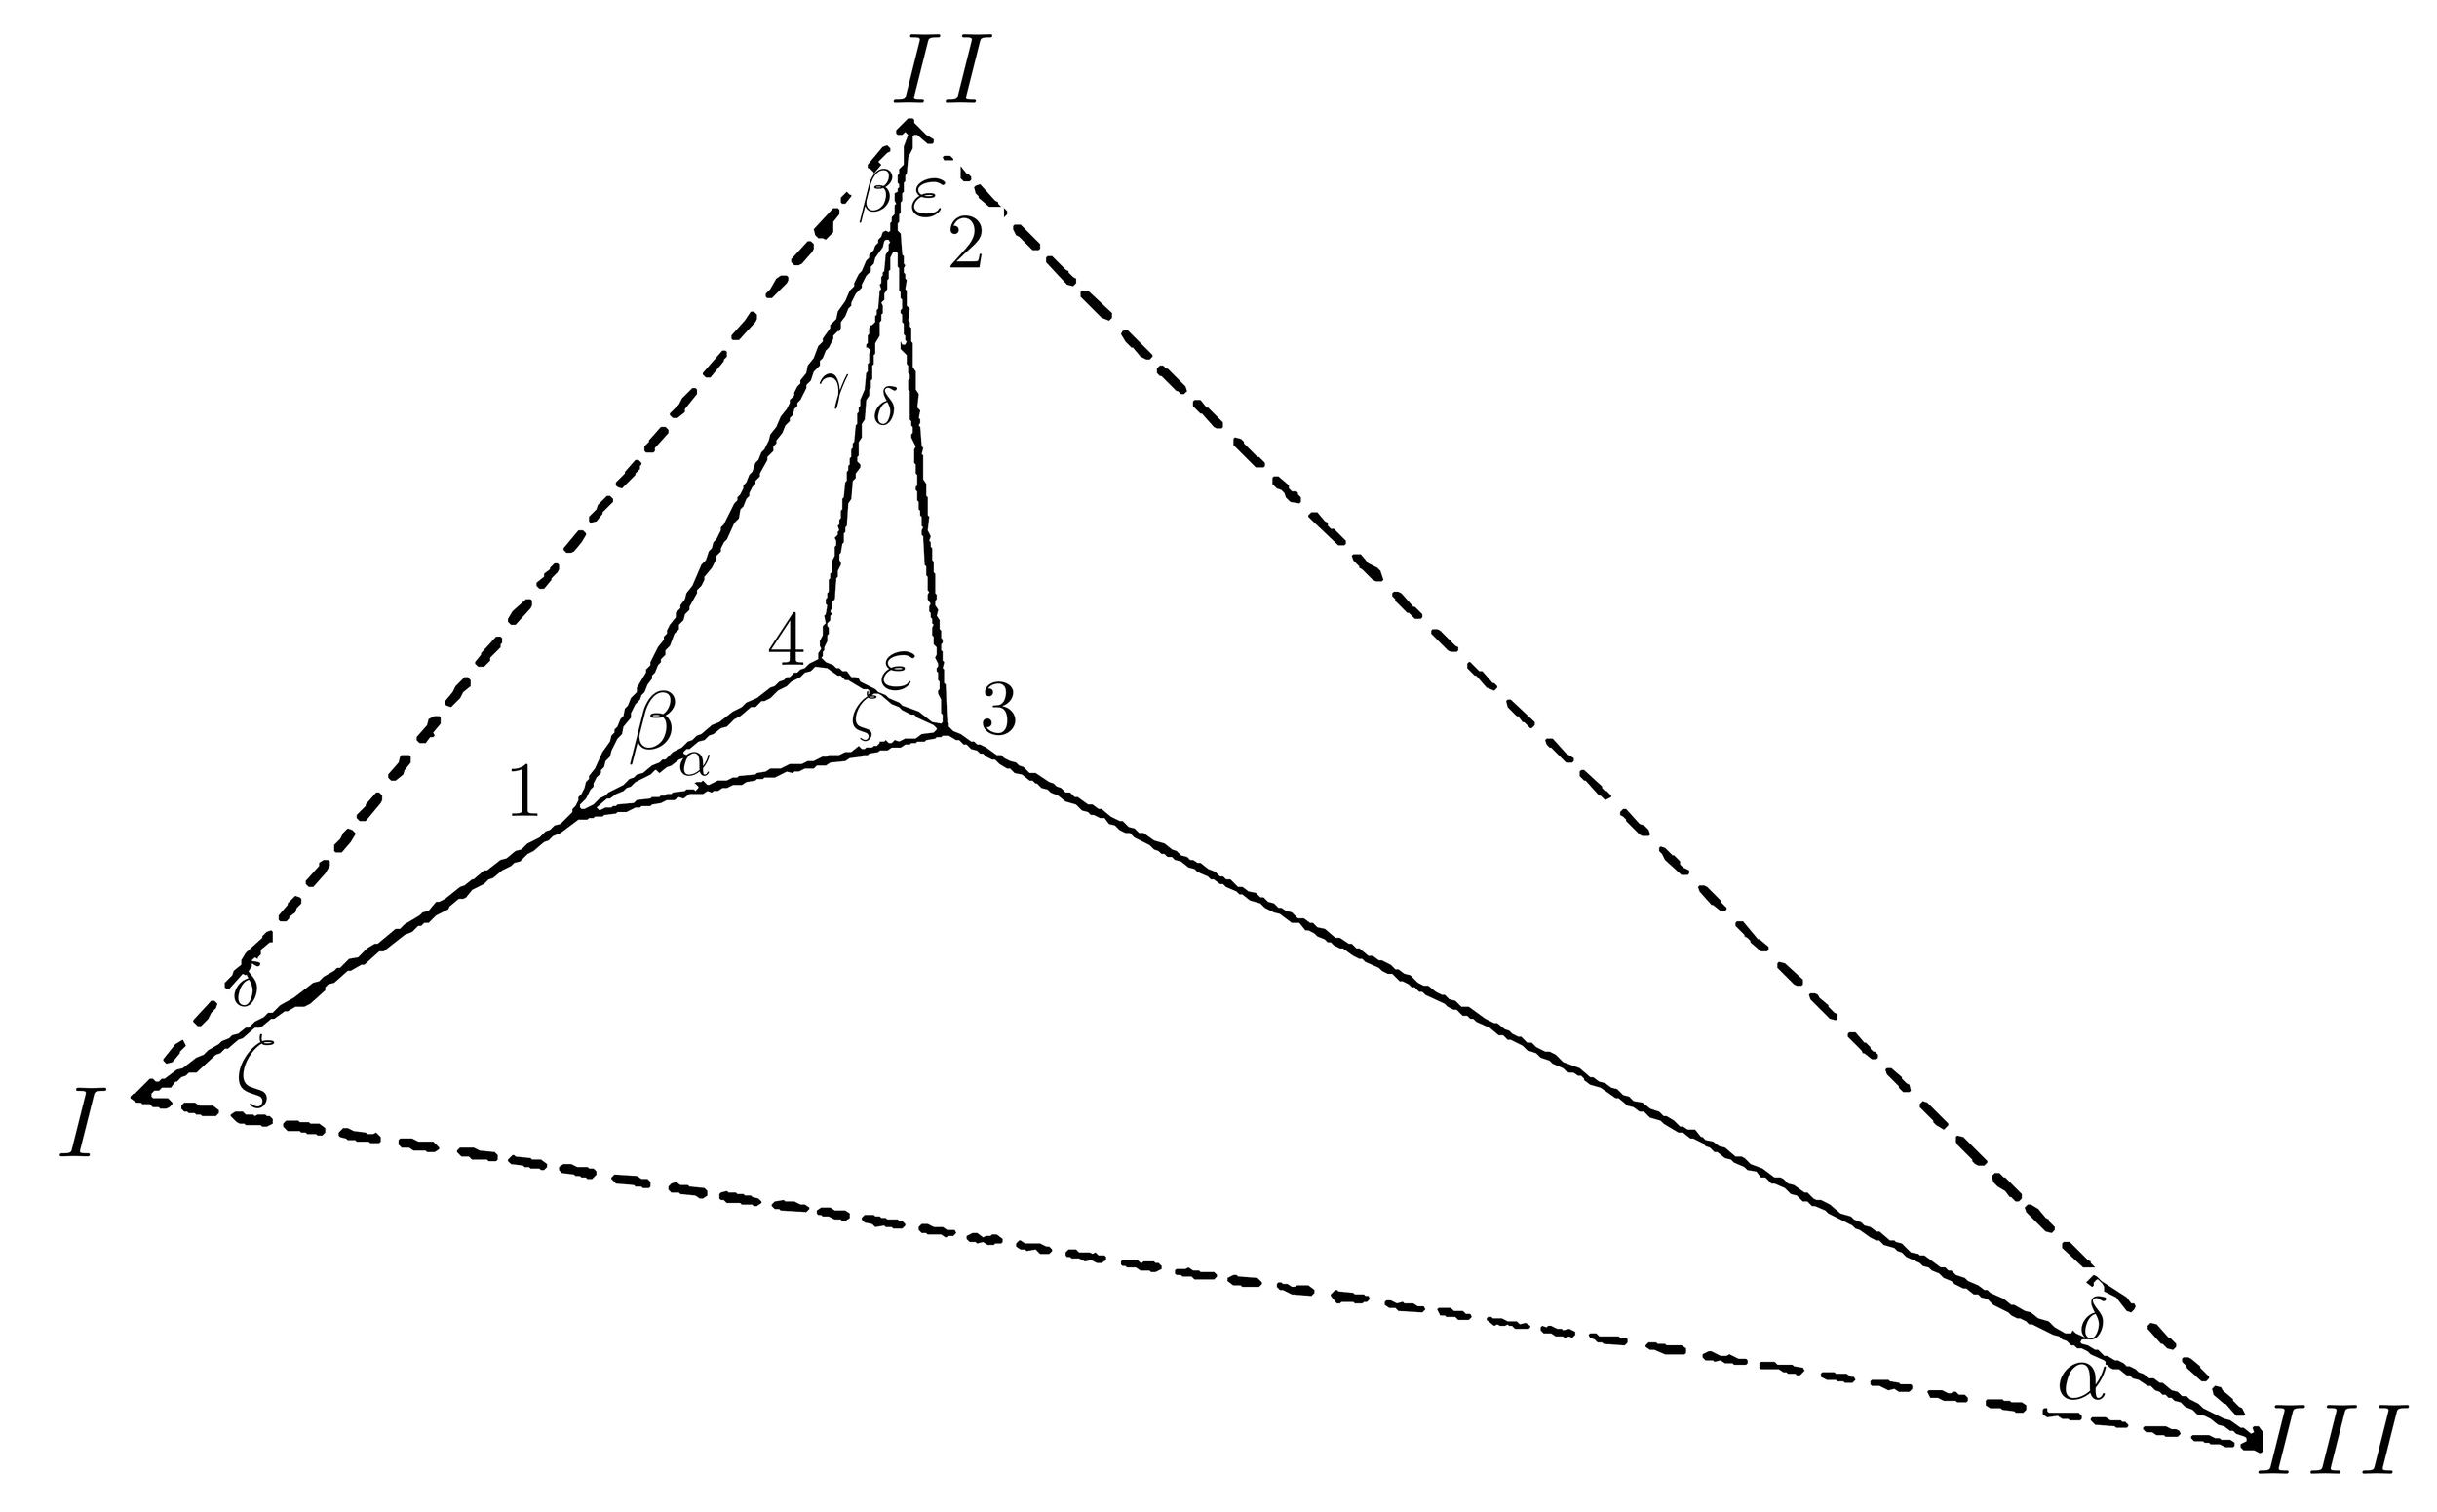
\begin{tikzpicture}[x=1pt,y=-1pt]
\path[use as bounding box] (0,0) rectangle (1606,989);
\path[fill=black,draw=none,even odd rule]
(1452,949) -- (1452,950) -- (1454,952) -- (1460,952) -- (1461,953) -- (1464,953) -- (1465,954) -- (1471,954) -- (1475,956) -- (1480,956) -- (1481,955) -- (1481,953) -- (1478,951) -- (1472,951) -- (1471,950) -- (1468,950) -- (1464,948) -- (1453,948) -- cycle
(1420,943) -- (1420,944) -- (1422,946) -- (1426,946) -- (1429,948) -- (1434,948) -- (1435,949) -- (1443,949) -- (1445,947) -- (1444,945) -- (1442,944) -- (1439,944) -- (1435,942) -- (1421,942) -- cycle
(1385,937) -- (1385,938) -- (1388,941) -- (1401,942) -- (1402,943) -- (1409,943) -- (1410,942) -- (1410,941) -- (1408,939) -- (1406,939) -- (1405,938) -- (1398,938) -- (1395,936) -- (1386,936) -- cycle
(1353,931) -- (1353,934) -- (1356,936) -- (1363,935) -- (1366,937) -- (1370,937) -- (1371,938) -- (1378,938) -- (1379,937) -- (1379,935) -- (1377,933) -- (1357,933) -- (1356,932) -- (1356,930) -- (1354,930) -- cycle
(1315,925) -- (1315,928) -- (1318,930) -- (1325,930) -- (1326,931) -- (1334,932) -- (1335,933) -- (1340,933) -- (1342,931) -- (1342,928) -- (1339,926) -- (1332,926) -- (1331,925) -- (1327,925) -- (1326,924) -- (1316,924) -- cycle
(1276,919) -- (1278,923) -- (1283,923) -- (1287,925) -- (1295,925) -- (1296,926) -- (1302,926) -- (1303,925) -- (1303,923) -- (1301,921) -- (1297,921) -- (1295,919) -- (1293,919) -- (1292,920) -- (1290,920) -- (1286,918) -- (1277,918) -- cycle
(1466,917) -- (1467,921) -- (1474,927) -- (1475,927) -- (1482,935) -- (1487,935) -- (1488,934) -- (1486,930) -- (1484,929) -- (1480,925) -- (1480,924) -- (1473,918) -- (1472,916) -- (1468,915) -- cycle
(1238,912) -- (1238,914) -- (1239,915) -- (1244,915) -- (1250,918) -- (1254,917) -- (1257,919) -- (1264,919) -- (1266,917) -- (1266,915) -- (1265,914) -- (1258,914) -- (1257,913) -- (1251,912) -- (1250,911) -- (1239,911) -- cycle
(1205,907) -- (1205,909) -- (1209,911) -- (1215,911) -- (1216,912) -- (1220,912) -- (1221,913) -- (1226,913) -- (1228,911) -- (1227,909) -- (1225,909) -- (1222,907) -- (1215,907) -- (1214,906) -- (1206,906) -- cycle
(1164,900) -- (1164,903) -- (1165,904) -- (1177,904) -- (1180,906) -- (1182,906) -- (1183,907) -- (1188,907) -- (1189,908) -- (1191,908) -- (1194,905) -- (1193,903) -- (1187,902) -- (1186,901) -- (1176,901) -- (1174,899) -- (1165,899) -- cycle
(1446,897) -- (1446,899) -- (1449,902) -- (1449,903) -- (1459,912) -- (1462,912) -- (1464,910) -- (1464,909) -- (1458,903) -- (1458,902) -- (1452,897) -- (1450,896) -- (1447,896) -- cycle
(1126,894) -- (1126,896) -- (1128,898) -- (1133,898) -- (1134,899) -- (1138,898) -- (1141,900) -- (1146,900) -- (1147,901) -- (1155,901) -- (1156,900) -- (1156,898) -- (1155,897) -- (1150,897) -- (1144,894) -- (1142,895) -- (1138,895) -- (1132,892) -- (1130,892) -- cycle
(1088,888) -- (1088,889) -- (1091,891) -- (1094,891) -- (1101,894) -- (1114,894) -- (1115,893) -- (1115,890) -- (1112,888) -- (1102,888) -- (1101,887) -- (1096,887) -- (1095,886) -- (1090,886) -- cycle
(1050,881) -- (1051,883) -- (1054,884) -- (1056,886) -- (1059,886) -- (1060,887) -- (1074,888) -- (1076,886) -- (1076,884) -- (1075,883) -- (1071,883) -- (1070,882) -- (1057,882) -- (1055,880) -- (1051,880) -- cycle
(1018,876) -- (1018,878) -- (1020,880) -- (1025,880) -- (1028,882) -- (1033,882) -- (1034,883) -- (1037,882) -- (1039,883) -- (1041,881) -- (1041,879) -- (1037,877) -- (1033,878) -- (1032,877) -- (1029,877) -- (1025,875) -- (1023,875) -- (1022,876) -- (1019,875) -- cycle
(1425,873) -- (1423,875) -- (1423,877) -- (1432,887) -- (1433,887) -- (1436,890) -- (1440,891) -- (1442,889) -- (1442,887) -- (1438,883) -- (1437,883) -- (1429,874) -- cycle
(982,870) -- (982,871) -- (987,875) -- (989,874) -- (991,875) -- (994,875) -- (996,874) -- (997,875) -- (999,875) -- (1001,877) -- (1010,877) -- (1011,876) -- (1011,875) -- (1008,873) -- (1004,874) -- (1002,872) -- (996,872) -- (992,870) -- (986,870) -- (985,869) -- (983,869) -- cycle
(949,864) -- (951,868) -- (954,868) -- (955,869) -- (961,869) -- (963,871) -- (970,871) -- (972,869) -- (971,867) -- (968,867) -- (966,865) -- (960,865) -- (958,863) -- (950,863) -- cycle
(914,859) -- (914,861) -- (917,863) -- (921,863) -- (923,865) -- (939,866) -- (941,864) -- (940,862) -- (936,862) -- (933,860) -- (927,860) -- (926,859) -- (922,860) -- (918,858) -- (915,858) -- cycle
(878,854) -- (878,855) -- (882,860) -- (884,860) -- (885,859) -- (893,859) -- (894,860) -- (899,860) -- (900,859) -- (902,859) -- (904,857) -- (903,855) -- (901,855) -- (900,854) -- (894,854) -- (893,853) -- (883,852) -- (882,851) -- (881,851) -- cycle
(842,847) -- (842,849) -- (844,851) -- (846,851) -- (852,854) -- (865,855) -- (867,853) -- (867,851) -- (863,848) -- (855,848) -- (854,849) -- (852,849) -- (849,847) -- (846,847) -- (845,846) -- (843,846) -- cycle
(1382,846) -- (1386,849) -- (1387,848) -- (1387,846) -- (1389,844) -- (1390,844) -- (1393,847) -- (1394,849) -- (1394,852) -- (1402,856) -- (1409,865) -- (1412,866) -- (1414,864) -- (1415,862) -- (1414,860) -- (1412,860) -- (1409,856) -- (1392,845) -- (1389,842) -- (1387,841) -- cycle
(809,843) -- (809,845) -- (813,848) -- (818,848) -- (819,849) -- (830,849) -- (832,847) -- (832,846) -- (829,843) -- (816,842) -- (815,841) -- (813,841) -- cycle
(774,838) -- (774,840) -- (775,841) -- (778,841) -- (779,842) -- (785,842) -- (787,844) -- (800,844) -- (802,842) -- (802,841) -- (800,839) -- (791,839) -- (790,838) -- (786,838) -- (783,836) -- (781,837) -- (775,837) -- cycle
(738,832) -- (738,834) -- (739,835) -- (741,835) -- (742,836) -- (748,836) -- (751,838) -- (757,838) -- (758,839) -- (761,839) -- (765,837) -- (765,835) -- (763,833) -- (761,833) -- (760,832) -- (753,832) -- (752,833) -- (751,833) -- (749,831) -- (739,831) -- cycle
(701,826) -- (701,828) -- (702,829) -- (704,829) -- (705,830) -- (710,830) -- (714,832) -- (718,831) -- (722,833) -- (725,833) -- (728,831) -- (728,829) -- (727,828) -- (723,828) -- (721,826) -- (719,827) -- (717,826) -- (710,826) -- (708,824) -- (703,824) -- cycle
(1366,820) -- (1366,823) -- (1380,836) -- (1388,836) -- (1385,833) -- (1385,832) -- (1383,831) -- (1371,819) -- (1367,819) -- cycle
(668,820) -- (668,822) -- (671,824) -- (674,824) -- (675,825) -- (681,824) -- (684,827) -- (690,827) -- (692,825) -- (692,824) -- (690,822) -- (688,822) -- (684,820) -- (674,820) -- (671,818) -- (670,818) -- cycle
(635,815) -- (635,817) -- (637,819) -- (641,819) -- (642,820) -- (646,819) -- (649,821) -- (653,821) -- (654,820) -- (658,820) -- (659,819) -- (659,817) -- (655,814) -- (652,814) -- (651,815) -- (648,815) -- (646,816) -- (642,813) -- (639,813) -- cycle
(603,809) -- (603,811) -- (605,813) -- (608,813) -- (609,814) -- (618,814) -- (621,816) -- (623,815) -- (626,815) -- (628,813) -- (627,811) -- (622,811) -- (619,809) -- (613,809) -- (609,807) -- (605,807) -- cycle
(565,803) -- (565,804) -- (567,806) -- (572,807) -- (574,809) -- (580,808) -- (581,809) -- (585,809) -- (586,810) -- (592,810) -- (594,808) -- (594,807) -- (592,805) -- (590,805) -- (589,804) -- (582,804) -- (581,803) -- (578,803) -- (577,802) -- (574,802) -- (573,801) -- (567,801) -- cycle
(535,798) -- (535,800) -- (536,801) -- (538,801) -- (539,802) -- (543,802) -- (547,804) -- (551,804) -- (552,805) -- (554,805) -- (557,803) -- (557,800) -- (554,798) -- (547,798) -- (544,796) -- (538,796) -- cycle
(1343,794) -- (1341,796) -- (1342,799) -- (1355,812) -- (1359,813) -- (1361,811) -- (1361,809) -- (1357,805) -- (1357,804) -- (1355,803) -- (1350,797) -- (1345,794) -- cycle
(505,794) -- (505,795) -- (507,797) -- (510,797) -- (511,798) -- (528,799) -- (530,797) -- (530,796) -- (527,794) -- (524,794) -- (520,792) -- (514,792) -- (513,791) -- (507,792) -- cycle
(470,787) -- (470,790) -- (471,791) -- (473,791) -- (475,793) -- (484,793) -- (485,794) -- (492,794) -- (493,795) -- (495,795) -- (498,793) -- (498,792) -- (496,790) -- (492,789) -- (491,788) -- (487,788) -- (486,787) -- (482,787) -- (481,786) -- (476,786) -- (475,785) -- (471,786) -- cycle
(436,782) -- (436,784) -- (438,786) -- (443,786) -- (444,787) -- (454,788) -- (457,790) -- (459,790) -- (462,788) -- (462,785) -- (460,783) -- (450,782) -- (449,781) -- (444,781) -- (441,779) -- (438,780) -- cycle
(398,776) -- (398,777) -- (401,780) -- (413,781) -- (414,782) -- (418,782) -- (419,783) -- (423,783) -- (424,782) -- (424,779) -- (422,777) -- (418,777) -- (415,775) -- (400,774) -- cycle
(1321,773) -- (1319,775) -- (1320,779) -- (1323,782) -- (1328,785) -- (1331,789) -- (1332,789) -- (1335,792) -- (1337,792) -- (1339,790) -- (1339,787) -- (1328,776) -- (1327,776) -- (1324,773) -- cycle
(363,769) -- (363,771) -- (365,773) -- (373,774) -- (374,775) -- (377,775) -- (378,776) -- (381,776) -- (382,777) -- (385,777) -- (388,774) -- (388,772) -- (386,770) -- (383,770) -- (382,769) -- (375,769) -- (371,767) -- (366,767) -- cycle
(329,764) -- (329,765) -- (331,767) -- (339,768) -- (340,769) -- (343,769) -- (344,770) -- (350,770) -- (351,771) -- (353,771) -- (355,769) -- (355,767) -- (351,764) -- (345,764) -- (344,763) -- (334,762) -- (333,761) -- (332,761) -- cycle
(295,758) -- (295,759) -- (298,762) -- (303,762) -- (305,764) -- (315,764) -- (316,765) -- (321,765) -- (322,764) -- (322,761) -- (320,759) -- (310,758) -- (306,756) -- (297,756) -- cycle
(256,751) -- (256,754) -- (258,756) -- (263,756) -- (266,758) -- (274,758) -- (275,759) -- (280,759) -- (283,757) -- (283,756) -- (279,752) -- (269,752) -- (265,750) -- (257,750) -- cycle
(1296,748) -- (1295,749) -- (1295,752) -- (1296,754) -- (1306,764) -- (1306,765) -- (1308,767) -- (1310,768) -- (1314,768) -- (1316,766) -- (1316,765) -- (1300,749) -- cycle
(216,746) -- (216,748) -- (217,749) -- (221,750) -- (222,751) -- (227,751) -- (228,752) -- (236,752) -- (237,753) -- (243,753) -- (244,752) -- (244,749) -- (241,746) -- (239,747) -- (235,747) -- (234,746) -- (226,745) -- (222,743) -- (219,743) -- cycle
(179,740) -- (179,742) -- (182,745) -- (190,745) -- (191,746) -- (194,746) -- (195,747) -- (201,747) -- (202,748) -- (205,748) -- (207,746) -- (207,743) -- (203,740) -- (197,740) -- (196,739) -- (190,739) -- (189,738) -- (181,738) -- cycle
(144,734) -- (144,735) -- (148,739) -- (150,740) -- (153,740) -- (154,741) -- (164,741) -- (165,742) -- (168,742) -- (172,740) -- (172,737) -- (170,735) -- (168,735) -- (167,734) -- (162,734) -- (160,735) -- (159,734) -- (154,734) -- (152,732) -- (147,732) -- cycle
(111,728) -- (111,730) -- (113,732) -- (115,732) -- (116,733) -- (120,733) -- (121,734) -- (124,734) -- (125,735) -- (134,735) -- (136,733) -- (136,731) -- (132,728) -- (123,728) -- (120,726) -- (113,726) -- cycle
(1273,725) -- (1271,727) -- (1271,729) -- (1280,738) -- (1280,739) -- (1282,741) -- (1287,744) -- (1290,741) -- (1290,740) -- (1276,726) -- cycle
(1249,703) -- (1248,704) -- (1249,707) -- (1257,715) -- (1257,716) -- (1260,719) -- (1264,719) -- (1265,718) -- (1264,714) -- (1262,713) -- (1259,710) -- (1259,709) -- (1252,703) -- cycle
(112,684) -- (107,687) -- (99,697) -- (99,698) -- (101,700) -- (105,699) -- (110,693) -- (110,692) -- (114,688) -- cycle
(1223,680) -- (1223,682) -- (1232,691) -- (1233,693) -- (1234,693) -- (1239,697) -- (1242,697) -- (1243,696) -- (1243,694) -- (1241,692) -- (1240,692) -- (1238,690) -- (1238,689) -- (1235,686) -- (1234,686) -- (1228,679) -- (1224,679) -- cycle
(133,658) -- (131,658) -- (119,671) -- (119,672) -- (122,675) -- (124,675) -- (129,670) -- (131,666) -- (134,663) -- (135,660) -- cycle
(1198,653) -- (1197,654) -- (1198,657) -- (1211,670) -- (1215,671) -- (1216,670) -- (1216,667) -- (1214,666) -- (1210,662) -- (1210,661) -- (1204,656) -- (1203,654) -- (1201,653) -- cycle
(1177,632) -- (1176,633) -- (1176,636) -- (1187,647) -- (1189,648) -- (1192,648) -- (1193,647) -- (1193,644) -- (1181,633) -- cycle
(171,611) -- (168,612) -- (165,615) -- (165,616) -- (154,626) -- (151,631) -- (151,634) -- (146,638) -- (145,641) -- (140,646) -- (140,649) -- (141,650) -- (143,650) -- (152,640) -- (154,641) -- (158,635) -- (158,631) -- (160,629) -- (162,630) -- (162,629) -- (164,627) -- (164,624) -- (170,619) -- (172,619) -- (172,612) -- cycle
(1148,606) -- (1148,608) -- (1154,614) -- (1154,615) -- (1156,616) -- (1158,618) -- (1158,619) -- (1165,625) -- (1169,625) -- (1170,624) -- (1170,622) -- (1164,617) -- (1163,617) -- (1153,605) -- (1149,605) -- cycle
(190,589) -- (187,588) -- (182,593) -- (182,594) -- (176,601) -- (176,604) -- (177,605) -- (181,605) -- (183,603) -- (183,602) -- (187,599) -- (188,596) -- (191,593) -- (191,590) -- cycle
(1123,582) -- (1124,585) -- (1132,594) -- (1133,594) -- (1138,598) -- (1141,598) -- (1142,597) -- (1142,596) -- (1138,592) -- (1138,591) -- (1129,582) -- (1127,581) -- (1124,581) -- cycle
(209,564) -- (206,564) -- (203,566) -- (203,568) -- (194,578) -- (194,580) -- (196,582) -- (199,582) -- (207,573) -- (210,568) -- (210,565) -- cycle
(1098,555) -- (1097,556) -- (1097,558) -- (1099,560) -- (1101,564) -- (1112,574) -- (1116,574) -- (1117,573) -- (1117,571) -- (1113,569) -- (1111,567) -- (1111,565) -- (1107,561) -- (1106,561) -- (1101,556) -- cycle
(225,544) -- (222,543) -- (219,546) -- (217,550) -- (213,554) -- (213,558) -- (214,559) -- (218,559) -- (224,552) -- (227,547) -- (227,546) -- cycle
(1071,532) -- (1071,534) -- (1073,535) -- (1075,537) -- (1075,538) -- (1084,547) -- (1086,548) -- (1090,548) -- (1091,547) -- (1090,544) -- (1087,541) -- (1084,540) -- (1075,530) -- (1073,530) -- cycle
(243,519) -- (241,519) -- (234,527) -- (234,528) -- (228,534) -- (228,536) -- (230,538) -- (234,538) -- (244,526) -- (245,524) -- (245,521) -- cycle
(1044,505) -- (1044,508) -- (1047,511) -- (1048,511) -- (1057,521) -- (1058,521) -- (1061,524) -- (1065,522) -- (1065,521) -- (1062,518) -- (1061,518) -- (1059,516) -- (1059,515) -- (1047,504) -- (1045,504) -- cycle
(263,494) -- (258,494) -- (257,495) -- (256,499) -- (249,507) -- (249,509) -- (251,511) -- (254,511) -- (259,507) -- (260,504) -- (264,499) -- (264,495) -- cycle
(1021,484) -- (1022,487) -- (1024,489) -- (1025,489) -- (1035,499) -- (1039,499) -- (1040,498) -- (1040,496) -- (1035,493) -- (1026,483) -- (1022,483) -- cycle
(283,468) -- (280,468) -- (276,470) -- (275,474) -- (268,482) -- (268,484) -- (270,486) -- (274,486) -- (277,482) -- (279,482) -- (280,481) -- (279,479) -- (284,473) -- (284,469) -- cycle
(996,457) -- (995,458) -- (996,462) -- (1002,468) -- (1003,468) -- (1006,472) -- (1007,472) -- (1011,476) -- (1012,476) -- (1014,474) -- (1014,472) -- (998,457) -- cycle
(302,442) -- (300,442) -- (294,448) -- (292,452) -- (287,458) -- (287,460) -- (288,461) -- (291,462) -- (297,456) -- (299,452) -- (304,448) -- (304,444) -- cycle
(970,432) -- (969,433) -- (969,436) -- (974,441) -- (975,441) -- (982,449) -- (987,451) -- (989,449) -- (989,448) -- (987,446) -- (986,446) -- (979,438) -- (977,438) -- (971,432) -- cycle
(324,415) -- (321,415) -- (311,426) -- (311,427) -- (307,432) -- (307,433) -- (309,435) -- (313,435) -- (317,431) -- (317,429) -- (324,422) -- (324,420) -- (325,419) -- (325,416) -- cycle
(945,411) -- (945,413) -- (956,424) -- (958,425) -- (962,425) -- (963,424) -- (963,422) -- (961,421) -- (951,411) -- (949,410) -- (946,410) -- cycle
(344,390) -- (341,390) -- (332,398) -- (329,403) -- (329,405) -- (331,407) -- (334,407) -- (344,396) -- (345,394) -- (345,391) -- cycle
(919,386) -- (919,388) -- (921,390) -- (921,391) -- (929,399) -- (930,399) -- (934,403) -- (938,403) -- (939,402) -- (939,400) -- (934,395) -- (933,395) -- (925,386) -- (923,385) -- (920,385) -- cycle
(362,366) -- (360,366) -- (357,369) -- (357,370) -- (353,373) -- (353,375) -- (348,379) -- (348,381) -- (350,383) -- (353,383) -- (358,377) -- (358,376) -- (362,372) -- (363,370) -- (363,367) -- cycle
(892,361) -- (893,364) -- (897,368) -- (897,369) -- (899,370) -- (906,377) -- (908,378) -- (912,378) -- (913,377) -- (911,371) -- (909,369) -- (903,366) -- (898,360) -- (893,360) -- cycle
(379,344) -- (376,344) -- (366,356) -- (366,357) -- (368,359) -- (371,359) -- (373,358) -- (378,352) -- (381,347) -- (381,346) -- cycle
(863,334) -- (863,335) -- (883,354) -- (887,354) -- (888,353) -- (888,351) -- (880,343) -- (878,343) -- (876,341) -- (876,339) -- (874,338) -- (869,332) -- (865,332) -- cycle
(397,321) -- (395,321) -- (389,327) -- (388,330) -- (383,335) -- (383,338) -- (384,339) -- (388,338) -- (392,333) -- (392,332) -- (399,325) -- (399,323) -- cycle
(840,308) -- (839,309) -- (839,313) -- (842,316) -- (845,317) -- (847,319) -- (848,322) -- (851,325) -- (857,326) -- (858,325) -- (858,322) -- (856,320) -- (856,319) -- (855,318) -- (852,318) -- (850,316) -- (850,314) -- (843,308) -- cycle
(416,297) -- (414,297) -- (407,305) -- (407,306) -- (401,312) -- (401,314) -- (402,315) -- (405,316) -- (414,307) -- (414,306) -- (417,303) -- (417,301) -- (418,300) -- (418,299) -- cycle
(814,282) -- (813,283) -- (813,287) -- (828,302) -- (833,302) -- (834,301) -- (834,299) -- (830,295) -- (829,295) -- (820,286) -- (820,285) -- (818,283) -- cycle
(434,275) -- (431,275) -- (423,284) -- (423,285) -- (420,288) -- (420,291) -- (421,292) -- (426,292) -- (427,291) -- (427,289) -- (436,279) -- (436,277) -- cycle
(787,257) -- (786,258) -- (786,261) -- (791,266) -- (792,266) -- (800,275) -- (802,276) -- (805,276) -- (806,275) -- (806,272) -- (796,262) -- (795,262) -- (791,257) -- cycle
(454,249) -- (452,249) -- (445,256) -- (443,260) -- (437,266) -- (437,267) -- (439,269) -- (442,269) -- (447,265) -- (447,263) -- (455,253) -- (455,250) -- cycle
(764,234) -- (762,236) -- (762,239) -- (764,241) -- (765,241) -- (775,251) -- (776,251) -- (778,253) -- (780,253) -- (782,251) -- (781,248) -- (769,236) -- (768,236) -- (766,234) -- cycle
(474,224) -- (472,224) -- (459,239) -- (459,240) -- (461,242) -- (464,242) -- (473,231) -- (473,230) -- (475,228) -- (475,225) -- cycle
(739,211) -- (738,213) -- (741,218) -- (745,222) -- (746,222) -- (751,228) -- (755,230) -- (757,230) -- (759,228) -- (759,227) -- (742,210) -- cycle
(493,198) -- (491,198) -- (487,204) -- (478,214) -- (478,216) -- (479,217) -- (483,217) -- (494,205) -- (495,203) -- (495,200) -- cycle
(712,184) -- (711,185) -- (711,188) -- (725,202) -- (730,204) -- (732,202) -- (732,199) -- (716,184) -- cycle
(515,174) -- (511,174) -- (508,176) -- (504,183) -- (501,186) -- (501,188) -- (502,189) -- (505,189) -- (515,179) -- (516,177) -- (516,175) -- cycle
(689,161) -- (688,162) -- (688,165) -- (702,180) -- (706,181) -- (708,179) -- (708,176) -- (706,175) -- (703,172) -- (703,171) -- (701,170) -- (692,161) -- cycle
(531,151) -- (529,151) -- (518,163) -- (518,165) -- (520,167) -- (523,167) -- (525,166) -- (532,158) -- (533,156) -- (533,153) -- cycle
(667,140) -- (666,141) -- (666,143) -- (668,147) -- (670,148) -- (679,157) -- (683,157) -- (684,156) -- (684,153) -- (671,140) -- cycle
(549,129) -- (546,129) -- (533,143) -- (534,147) -- (536,149) -- (539,149) -- (541,150) -- (546,145) -- (546,138) -- (550,133) -- (550,130) -- cycle
(555,118) -- (551,122) -- (551,125) -- (552,126) -- (554,126) -- (558,121) -- (558,120) -- (557,120) -- cycle
(641,114) -- (640,115) -- (641,119) -- (643,121) -- (643,122) -- (650,128) -- (659,128) -- (660,129) -- (660,135) -- (662,133) -- (662,131) -- (659,128) -- (658,128) -- (656,126) -- (656,125) -- (654,124) -- (644,113) -- cycle
(631,101) -- (631,109) -- (633,111) -- (637,111) -- (638,110) -- (638,108) -- (636,106) -- (635,106) -- cycle
(619,95) -- (620,97) -- (626,97) -- (626,96) -- (624,94) -- (620,94) -- cycle
(582,87) -- (579,88) -- (569,100) -- (569,102) -- (571,103) -- (573,105) -- (573,106) -- (578,100) -- (576,98) -- (582,92) -- (584,91) -- (584,89) -- cycle
(77,722) -- (77,723) -- (81,726) -- (84,726) -- (85,727) -- (90,727) -- (92,729) -- (96,729) -- (97,730) -- (101,730) -- (103,729) -- (105,727) -- (105,726) -- (102,723) -- (92,723) -- (91,722) -- (91,720) -- (93,718) -- (96,718) -- (98,716) -- (104,716) -- (107,712) -- (108,712) -- (111,709) -- (114,708) -- (116,706) -- (121,706) -- (134,694) -- (137,693) -- (140,690) -- (142,690) -- (149,684) -- (152,683) -- (160,676) -- (163,676) -- (165,675) -- (171,670) -- (173,670) -- (180,665) -- (182,665) -- (187,662) -- (193,662) -- (197,660) -- (207,651) -- (207,649) -- (209,647) -- (213,646) -- (222,638) -- (224,638) -- (231,634) -- (233,634) -- (243,625) -- (246,625) -- (260,614) -- (265,612) -- (269,608) -- (271,608) -- (273,606) -- (276,606) -- (281,601) -- (289,597) -- (290,595) -- (296,590) -- (299,590) -- (301,589) -- (305,584) -- (313,580) -- (316,577) -- (319,576) -- (325,571) -- (331,568) -- (333,566) -- (337,565) -- (342,560) -- (346,558) -- (353,552) -- (356,551) -- (359,548) -- (364,546) -- (376,537) -- (382,537) -- (383,536) -- (386,536) -- (387,535) -- (392,535) -- (393,534) -- (401,533) -- (402,532) -- (408,532) -- (414,529) -- (417,529) -- (418,528) -- (424,528) -- (425,527) -- (431,526) -- (435,524) -- (440,524) -- (443,522) -- (446,523) -- (450,520) -- (459,520) -- (462,518) -- (465,519) -- (466,518) -- (469,518) -- (472,516) -- (475,516) -- (479,514) -- (485,514) -- (488,512) -- (494,511) -- (495,510) -- (499,510) -- (500,509) -- (507,509) -- (515,505) -- (519,506) -- (520,505) -- (523,505) -- (527,503) -- (533,503) -- (535,501) -- (541,501) -- (544,499) -- (554,498) -- (557,496) -- (565,495) -- (566,494) -- (569,494) -- (570,493) -- (576,492) -- (577,491) -- (582,491) -- (585,489) -- (591,489) -- (594,487) -- (597,487) -- (598,486) -- (601,486) -- (602,485) -- (607,485) -- (608,484) -- (614,483) -- (615,482) -- (618,482) -- (619,481) -- (623,481) -- (628,484) -- (630,484) -- (633,487) -- (635,487) -- (638,490) -- (642,491) -- (644,493) -- (646,493) -- (648,495) -- (652,497) -- (654,497) -- (657,500) -- (662,503) -- (664,503) -- (667,506) -- (672,507) -- (677,511) -- (679,511) -- (681,513) -- (682,513) -- (685,516) -- (689,517) -- (691,519) -- (696,521) -- (701,525) -- (708,527) -- (712,531) -- (716,532) -- (718,534) -- (720,534) -- (724,536) -- (727,536) -- (730,540) -- (734,541) -- (737,544) -- (741,546) -- (744,546) -- (747,549) -- (757,554) -- (760,557) -- (763,558) -- (765,560) -- (767,560) -- (769,562) -- (772,562) -- (774,564) -- (778,565) -- (783,569) -- (787,570) -- (789,572) -- (796,575) -- (798,577) -- (800,577) -- (804,580) -- (806,580) -- (808,582) -- (815,585) -- (817,587) -- (819,587) -- (824,591) -- (831,593) -- (834,596) -- (840,599) -- (844,600) -- (852,606) -- (857,606) -- (861,611) -- (863,611) -- (867,613) -- (869,615) -- (874,617) -- (876,619) -- (878,619) -- (880,621) -- (884,623) -- (886,623) -- (893,628) -- (897,630) -- (899,630) -- (901,632) -- (910,636) -- (912,638) -- (916,640) -- (919,640) -- (924,645) -- (926,645) -- (930,647) -- (932,649) -- (934,649) -- (937,652) -- (939,652) -- (941,654) -- (954,660) -- (956,662) -- (960,664) -- (962,664) -- (966,668) -- (969,668) -- (971,670) -- (973,670) -- (975,672) -- (984,676) -- (990,681) -- (993,681) -- (996,684) -- (998,684) -- (1006,688) -- (1009,691) -- (1015,693) -- (1018,696) -- (1024,698) -- (1026,700) -- (1033,703) -- (1035,705) -- (1037,706) -- (1040,706) -- (1043,708) -- (1045,708) -- (1047,710) -- (1047,711) -- (1051,714) -- (1058,716) -- (1068,723) -- (1070,723) -- (1076,728) -- (1080,729) -- (1084,732) -- (1087,732) -- (1091,736) -- (1098,738) -- (1100,740) -- (1110,746) -- (1113,746) -- (1118,750) -- (1120,750) -- (1126,753) -- (1128,755) -- (1131,756) -- (1134,759) -- (1136,759) -- (1141,763) -- (1145,764) -- (1147,766) -- (1154,769) -- (1156,771) -- (1162,772) -- (1165,776) -- (1168,776) -- (1172,780) -- (1174,780) -- (1181,783) -- (1185,787) -- (1189,788) -- (1193,792) -- (1196,792) -- (1199,795) -- (1201,795) -- (1208,798) -- (1210,800) -- (1226,808) -- (1228,810) -- (1231,811) -- (1238,816) -- (1242,818) -- (1244,818) -- (1247,821) -- (1254,823) -- (1256,825) -- (1259,826) -- (1262,829) -- (1271,833) -- (1273,835) -- (1277,836) -- (1279,838) -- (1284,840) -- (1287,843) -- (1292,845) -- (1294,847) -- (1300,850) -- (1302,850) -- (1307,854) -- (1310,854) -- (1312,856) -- (1316,857) -- (1320,861) -- (1330,866) -- (1332,868) -- (1336,870) -- (1338,870) -- (1342,872) -- (1344,874) -- (1346,874) -- (1360,881) -- (1364,882) -- (1366,884) -- (1369,885) -- (1372,888) -- (1374,888) -- (1376,890) -- (1379,890) -- (1383,892) -- (1385,894) -- (1394,898) -- (1395,899) -- (1395,901) -- (1396,901) -- (1398,903) -- (1400,904) -- (1404,904) -- (1409,908) -- (1411,908) -- (1413,910) -- (1417,911) -- (1423,915) -- (1425,915) -- (1428,918) -- (1431,919) -- (1433,921) -- (1435,921) -- (1437,923) -- (1439,923) -- (1441,925) -- (1445,926) -- (1448,929) -- (1453,931) -- (1456,934) -- (1461,935) -- (1465,937) -- (1470,941) -- (1474,942) -- (1478,945) -- (1480,945) -- (1482,947) -- (1488,949) -- (1489,950) -- (1489,952) -- (1485,954) -- (1485,956) -- (1487,958) -- (1494,958) -- (1498,960) -- (1500,959) -- (1500,946) -- (1497,942) -- (1494,942) -- (1493,943) -- (1494,946) -- (1492,947) -- (1487,943) -- (1485,943) -- (1478,938) -- (1474,937) -- (1460,930) -- (1457,927) -- (1451,924) -- (1449,922) -- (1446,922) -- (1443,919) -- (1439,918) -- (1433,913) -- (1431,913) -- (1427,910) -- (1424,910) -- (1420,907) -- (1417,906) -- (1415,904) -- (1411,902) -- (1409,902) -- (1407,900) -- (1403,898) -- (1401,898) -- (1396,895) -- (1394,895) -- (1390,891) -- (1388,891) -- (1383,888) -- (1379,887) -- (1378,886) -- (1379,884) -- (1384,884) -- (1375,880) -- (1373,878) -- (1372,880) -- (1368,880) -- (1361,876) -- (1357,872) -- (1350,870) -- (1345,866) -- (1341,865) -- (1334,861) -- (1332,861) -- (1327,857) -- (1318,853) -- (1316,851) -- (1314,851) -- (1310,848) -- (1303,845) -- (1301,843) -- (1295,841) -- (1292,838) -- (1290,838) -- (1288,836) -- (1285,836) -- (1274,828) -- (1271,828) -- (1270,827) -- (1265,826) -- (1259,820) -- (1255,819) -- (1254,818) -- (1251,818) -- (1244,812) -- (1242,812) -- (1238,809) -- (1234,808) -- (1232,806) -- (1227,804) -- (1225,802) -- (1218,800) -- (1211,794) -- (1205,791) -- (1202,791) -- (1200,790) -- (1196,786) -- (1194,786) -- (1187,781) -- (1183,780) -- (1180,777) -- (1178,776) -- (1174,776) -- (1166,770) -- (1158,767) -- (1154,763) -- (1152,762) -- (1148,762) -- (1141,756) -- (1137,755) -- (1133,752) -- (1128,751) -- (1126,749) -- (1125,749) -- (1121,744) -- (1116,744) -- (1113,742) -- (1111,742) -- (1107,738) -- (1102,735) -- (1100,735) -- (1097,732) -- (1091,730) -- (1086,726) -- (1080,725) -- (1077,722) -- (1073,721) -- (1069,717) -- (1065,716) -- (1061,713) -- (1057,712) -- (1053,709) -- (1051,709) -- (1044,703) -- (1033,699) -- (1028,694) -- (1024,692) -- (1021,692) -- (1015,689) -- (1012,686) -- (1009,686) -- (1005,682) -- (1003,682) -- (999,680) -- (997,678) -- (994,677) -- (989,673) -- (987,673) -- (981,670) -- (970,662) -- (965,662) -- (961,658) -- (957,657) -- (954,654) -- (952,654) -- (948,652) -- (943,648) -- (940,648) -- (936,646) -- (931,641) -- (927,640) -- (923,637) -- (921,637) -- (918,634) -- (912,631) -- (910,631) -- (906,628) -- (903,628) -- (897,623) -- (895,623) -- (892,620) -- (890,620) -- (884,616) -- (881,616) -- (874,610) -- (869,609) -- (866,606) -- (864,606) -- (860,603) -- (856,603) -- (852,599) -- (848,598) -- (845,596) -- (843,596) -- (840,593) -- (836,592) -- (833,589) -- (831,589) -- (828,586) -- (823,585) -- (819,582) -- (816,582) -- (811,577) -- (808,577) -- (806,575) -- (804,575) -- (801,572) -- (796,570) -- (791,566) -- (789,566) -- (786,564) -- (784,564) -- (782,562) -- (778,561) -- (775,558) -- (772,557) -- (767,553) -- (760,551) -- (753,546) -- (750,546) -- (747,543) -- (743,542) -- (739,538) -- (737,538) -- (731,535) -- (725,530) -- (723,530) -- (719,527) -- (716,527) -- (709,522) -- (707,522) -- (704,519) -- (701,519) -- (698,516) -- (695,515) -- (693,513) -- (690,512) -- (681,506) -- (677,506) -- (673,502) -- (670,501) -- (668,499) -- (664,498) -- (660,496) -- (658,494) -- (655,494) -- (648,489) -- (644,487) -- (642,487) -- (640,485) -- (638,485) -- (631,480) -- (626,478) -- (623,475) -- (623,473) -- (622,472) -- (621,447) -- (620,446) -- (620,437) -- (619,436) -- (620,432) -- (619,431) -- (619,425) -- (618,424) -- (618,420) -- (619,419) -- (619,417) -- (618,416) -- (618,411) -- (617,410) -- (617,404) -- (615,401) -- (616,397) -- (614,394) -- (614,391) -- (615,390) -- (615,387) -- (614,386) -- (614,373) -- (613,372) -- (613,365) -- (612,364) -- (612,356) -- (611,355) -- (611,352) -- (610,351) -- (611,348) -- (609,344) -- (610,335) -- (609,334) -- (609,322) -- (608,321) -- (608,313) -- (606,310) -- (606,294) -- (605,293) -- (606,289) -- (605,288) -- (604,275) -- (603,274) -- (604,272) -- (604,270) -- (603,269) -- (604,264) -- (602,262) -- (603,253) -- (601,250) -- (601,238) -- (599,235) -- (599,219) -- (598,218) -- (598,209) -- (597,208) -- (597,205) -- (596,204) -- (597,196) -- (595,194) -- (595,184) -- (594,183) -- (595,177) -- (594,176) -- (594,173) -- (593,172) -- (593,169) -- (594,167) -- (593,166) -- (593,161) -- (592,160) -- (591,146) -- (589,144) -- (589,139) -- (590,138) -- (590,133) -- (591,132) -- (591,125) -- (592,124) -- (592,119) -- (593,118) -- (593,112) -- (594,111) -- (594,107) -- (595,106) -- (596,95) -- (599,89) -- (599,81) -- (600,80) -- (602,80) -- (609,86) -- (612,86) -- (613,85) -- (613,83) -- (608,80) -- (600,72) -- (600,70) -- (599,69) -- (596,69) -- (588,77) -- (588,79) -- (589,80) -- (592,80) -- (594,78) -- (596,80) -- (593,88) -- (593,100) -- (590,103) -- (590,106) -- (589,107) -- (589,112) -- (590,113) -- (590,115) -- (589,116) -- (589,118) -- (587,119) -- (587,124) -- (588,126) -- (587,127) -- (587,133) -- (585,135) -- (585,138) -- (584,139) -- (584,144) -- (583,145) -- (581,144) -- (579,145) -- (578,148) -- (576,150) -- (576,152) -- (574,154) -- (573,157) -- (570,160) -- (570,162) -- (568,164) -- (565,171) -- (563,173) -- (560,179) -- (560,181) -- (557,184) -- (554,191) -- (549,198) -- (548,203) -- (544,207) -- (544,209) -- (539,216) -- (539,218) -- (536,221) -- (533,229) -- (529,234) -- (528,239) -- (524,244) -- (524,246) -- (522,248) -- (520,252) -- (520,254) -- (517,257) -- (517,259) -- (515,263) -- (511,268) -- (508,275) -- (504,280) -- (503,284) -- (500,290) -- (498,292) -- (496,297) -- (494,299) -- (492,305) -- (490,307) -- (488,312) -- (486,314) -- (486,316) -- (484,320) -- (482,322) -- (482,324) -- (480,326) -- (473,340) -- (471,342) -- (471,344) -- (468,350) -- (466,352) -- (465,356) -- (463,358) -- (461,364) -- (458,367) -- (452,381) -- (448,386) -- (447,390) -- (444,394) -- (444,396) -- (441,399) -- (441,402) -- (437,407) -- (435,411) -- (435,413) -- (433,415) -- (433,417) -- (429,422) -- (424,432) -- (424,434) -- (421,437) -- (421,439) -- (415,449) -- (415,452) -- (411,456) -- (409,461) -- (407,463) -- (406,468) -- (404,470) -- (402,475) -- (400,477) -- (400,479) -- (398,481) -- (397,485) -- (392,492) -- (387,503) -- (383,508) -- (383,510) -- (381,512) -- (380,516) -- (378,520) -- (376,522) -- (376,524) -- (374,528) -- (372,530) -- (372,532) -- (364,540) -- (360,541) -- (357,544) -- (354,545) -- (350,549) -- (342,553) -- (338,557) -- (334,558) -- (328,563) -- (324,564) -- (315,571) -- (313,571) -- (306,577) -- (305,577) -- (300,581) -- (297,582) -- (287,590) -- (283,592) -- (281,592) -- (276,598) -- (272,599) -- (270,601) -- (260,607) -- (257,610) -- (254,610) -- (242,620) -- (240,620) -- (235,623) -- (229,629) -- (223,630) -- (217,636) -- (215,636) -- (213,638) -- (206,642) -- (203,645) -- (199,646) -- (186,656) -- (177,661) -- (172,666) -- (169,666) -- (166,669) -- (160,672) -- (156,676) -- (154,676) -- (149,680) -- (145,681) -- (143,683) -- (138,685) -- (136,687) -- (129,691) -- (126,694) -- (121,696) -- (112,703) -- (108,704) -- (100,710) -- (98,710) -- (96,712) -- (94,712) -- (92,710) -- (90,710) -- (80,720) -- (79,720) -- cycle
(615,476) -- (615,477) -- (613,479) -- (605,480) -- (601,483) -- (594,483) -- (590,485) -- (587,484) -- (585,486) -- (583,486) -- (581,484) -- (580,485) -- (577,485) -- (577,486) -- (575,488) -- (573,488) -- (572,489) -- (568,489) -- (567,490) -- (565,490) -- (563,488) -- (558,492) -- (554,492) -- (550,494) -- (543,494) -- (542,495) -- (539,495) -- (533,498) -- (529,498) -- (525,500) -- (517,500) -- (511,503) -- (504,503) -- (501,505) -- (495,506) -- (494,507) -- (483,508) -- (482,509) -- (479,509) -- (475,511) -- (469,511) -- (463,514) -- (462,514) -- (459,511) -- (458,512) -- (455,512) -- (453,513) -- (454,513) -- (456,515) -- (456,516) -- (454,518) -- (453,517) -- (448,517) -- (447,518) -- (439,519) -- (438,520) -- (435,520) -- (434,521) -- (431,521) -- (430,522) -- (425,522) -- (424,523) -- (415,524) -- (413,526) -- (402,527) -- (401,528) -- (399,528) -- (398,529) -- (394,529) -- (390,531) -- (388,529) -- (395,523) -- (397,523) -- (401,520) -- (406,518) -- (408,516) -- (411,515) -- (414,512) -- (424,507) -- (427,504) -- (428,504) -- (430,506) -- (435,502) -- (438,501) -- (443,497) -- (446,496) -- (448,494) -- (446,493) -- (446,492) -- (448,490) -- (450,490) -- (456,485) -- (460,484) -- (463,481) -- (466,480) -- (471,476) -- (475,475) -- (480,470) -- (484,468) -- (491,462) -- (494,462) -- (498,458) -- (500,458) -- (504,456) -- (509,451) -- (515,448) -- (518,445) -- (524,442) -- (527,439) -- (531,438) -- (534,435) -- (542,436) -- (549,441) -- (551,441) -- (554,444) -- (556,444) -- (566,450) -- (569,450) -- (570,451) -- (570,453) -- (569,454) -- (571,455) -- (573,453) -- (576,453) -- (578,454) -- (585,460) -- (590,462) -- (592,464) -- (598,467) -- (600,467) -- (602,469) -- (613,474) -- cycle
(586,158) -- (588,158) -- (589,159) -- (589,168) -- (590,169) -- (590,184) -- (591,185) -- (591,189) -- (592,190) -- (592,196) -- (591,197) -- (591,199) -- (592,200) -- (592,205) -- (593,206) -- (593,213) -- (594,214) -- (594,217) -- (595,218) -- (594,220) -- (592,220) -- (591,218) -- (591,223) -- (595,227) -- (595,233) -- (596,234) -- (596,239) -- (597,240) -- (597,243) -- (596,244) -- (596,250) -- (597,251) -- (597,270) -- (598,271) -- (598,274) -- (599,275) -- (599,279) -- (598,280) -- (598,282) -- (601,288) -- (600,290) -- (600,299) -- (601,300) -- (601,306) -- (602,307) -- (602,314) -- (601,315) -- (601,317) -- (602,318) -- (602,324) -- (603,325) -- (603,330) -- (604,331) -- (604,334) -- (605,335) -- (605,341) -- (606,342) -- (605,344) -- (605,347) -- (606,348) -- (607,367) -- (608,368) -- (608,374) -- (609,375) -- (609,384) -- (610,385) -- (609,387) -- (609,390) -- (611,393) -- (610,395) -- (610,398) -- (611,399) -- (611,402) -- (612,403) -- (612,406) -- (613,407) -- (612,409) -- (612,414) -- (613,415) -- (613,420) -- (615,422) -- (615,427) -- (614,429) -- (616,433) -- (616,435) -- (615,436) -- (615,438) -- (616,439) -- (616,444) -- (617,445) -- (617,450) -- (616,451) -- (616,453) -- (618,457) -- (618,466) -- (619,467) -- (619,472) -- (618,473) -- (612,472) -- (603,465) -- (592,461) -- (590,459) -- (583,456) -- (581,454) -- (576,452) -- (574,450) -- (564,445) -- (563,443) -- (561,442) -- (558,442) -- (555,438) -- (552,438) -- (550,436) -- (548,436) -- (546,434) -- (541,432) -- (538,429) -- (539,428) -- (539,425) -- (540,424) -- (540,422) -- (542,418) -- (542,414) -- (543,413) -- (543,409) -- (542,408) -- (542,406) -- (544,404) -- (544,401) -- (545,400) -- (544,398) -- (545,396) -- (545,392) -- (547,390) -- (548,376) -- (549,375) -- (549,371) -- (551,367) -- (551,365) -- (550,364) -- (550,360) -- (551,359) -- (552,353) -- (553,352) -- (553,346) -- (554,345) -- (554,342) -- (555,341) -- (556,326) -- (558,323) -- (559,311) -- (561,309) -- (561,306) -- (564,302) -- (564,300) -- (562,298) -- (562,295) -- (563,294) -- (563,285) -- (565,282) -- (565,273) -- (567,270) -- (568,257) -- (570,254) -- (570,250) -- (571,249) -- (571,244) -- (572,243) -- (572,234) -- (573,233) -- (573,227) -- (574,226) -- (574,219) -- (577,214) -- (577,205) -- (578,204) -- (578,200) -- (579,199) -- (579,194) -- (578,192) -- (580,190) -- (580,186) -- (582,183) -- (582,177) -- (583,176) -- (583,171) -- (584,170) -- (584,162) -- cycle
(583,150) -- (584,152) -- (583,153) -- (583,157) -- (581,160) -- (580,171) -- (579,172) -- (579,174) -- (578,175) -- (578,179) -- (577,180) -- (578,183) -- (577,184) -- (576,196) -- (575,197) -- (575,200) -- (574,201) -- (574,205) -- (572,207) -- (571,207) -- (570,209) -- (570,213) -- (569,214) -- (569,219) -- (568,220) -- (568,222) -- (569,222) -- (571,224) -- (570,226) -- (570,232) -- (569,233) -- (569,238) -- (568,239) -- (567,250) -- (564,257) -- (564,261) -- (563,262) -- (563,265) -- (562,266) -- (562,273) -- (561,274) -- (560,285) -- (559,286) -- (559,289) -- (558,290) -- (558,295) -- (557,296) -- (557,300) -- (556,301) -- (556,304) -- (555,305) -- (555,311) -- (554,312) -- (553,322) -- (552,323) -- (552,330) -- (551,331) -- (551,336) -- (550,337) -- (550,340) -- (549,341) -- (550,344) -- (549,345) -- (549,347) -- (547,349) -- (548,351) -- (548,354) -- (547,355) -- (547,361) -- (545,365) -- (545,372) -- (544,373) -- (544,376) -- (543,377) -- (543,385) -- (542,386) -- (542,389) -- (541,390) -- (541,393) -- (542,394) -- (541,400) -- (540,401) -- (541,406) -- (539,408) -- (539,414) -- (537,418) -- (537,421) -- (538,423) -- (536,426) -- (536,430) -- (530,433) -- (527,436) -- (524,437) -- (522,439) -- (520,439) -- (517,442) -- (515,442) -- (513,444) -- (510,445) -- (507,448) -- (504,449) -- (495,456) -- (488,459) -- (485,462) -- (479,465) -- (470,472) -- (465,474) -- (458,480) -- (455,481) -- (452,484) -- (449,485) -- (445,489) -- (439,492) -- (434,497) -- (432,497) -- (430,499) -- (425,501) -- (419,506) -- (415,507) -- (413,509) -- (410,510) -- (406,514) -- (396,519) -- (394,521) -- (390,523) -- (386,527) -- (380,530) -- (378,530) -- (377,529) -- (377,527) -- (381,523) -- (384,517) -- (386,515) -- (386,513) -- (388,509) -- (391,506) -- (391,504) -- (393,502) -- (394,498) -- (397,495) -- (398,491) -- (402,483) -- (405,480) -- (406,475) -- (411,469) -- (411,466) -- (414,460) -- (417,457) -- (418,454) -- (420,452) -- (422,447) -- (425,443) -- (425,441) -- (427,439) -- (429,434) -- (431,432) -- (431,430) -- (434,427) -- (434,424) -- (437,421) -- (440,413) -- (443,410) -- (443,407) -- (446,404) -- (447,400) -- (450,397) -- (450,395) -- (455,386) -- (455,384) -- (458,381) -- (460,377) -- (460,375) -- (465,369) -- (468,363) -- (468,361) -- (471,358) -- (471,356) -- (473,352) -- (475,350) -- (480,339) -- (483,336) -- (484,330) -- (486,328) -- (488,323) -- (490,321) -- (490,319) -- (492,315) -- (494,313) -- (494,311) -- (497,308) -- (497,306) -- (502,297) -- (502,295) -- (506,291) -- (506,288) -- (508,286) -- (508,284) -- (512,279) -- (514,274) -- (517,271) -- (517,269) -- (519,267) -- (520,263) -- (522,261) -- (522,259) -- (524,257) -- (528,249) -- (528,247) -- (531,244) -- (533,238) -- (537,234) -- (537,231) -- (539,229) -- (541,224) -- (543,222) -- (546,216) -- (546,214) -- (549,211) -- (550,211) -- (551,209) -- (551,205) -- (554,201) -- (556,196) -- (558,194) -- (558,192) -- (561,186) -- (565,182) -- (565,180) -- (568,174) -- (571,171) -- (571,168) -- (573,166) -- (574,162) -- (579,155) -- (580,151) -- (581,150) -- cycle;
\node[inner sep=0pt,font=\fontsize{10}{10}\selectfont] at (45,739) {\scalebox{6.7}{$I$}};
\node[inner sep=0pt,font=\fontsize{10}{10}\selectfont] at (619,36) {\scalebox{6.7}{$II$}};
\node[inner sep=0pt,font=\fontsize{10}{10}\selectfont] at (1547,951) {\scalebox{6.7}{$III$}};
\node[inner sep=0pt,font=\fontsize{10}{10}\selectfont] at (340,518) {\scalebox{5.2}{$1$}};
\node[inner sep=0pt,font=\fontsize{10}{10}\selectfont] at (635,152) {\scalebox{5.2}{$2$}};
\node[inner sep=0pt,font=\fontsize{10}{10}\selectfont] at (657,463) {\scalebox{5.2}{$3$}};
\node[inner sep=0pt,font=\fontsize{10}{10}\selectfont] at (515,417) {\scalebox{5.2}{$4$}};
\node[inner sep=0pt,font=\fontsize{10}{10}\selectfont] at (426,476) {\scalebox{5.5}{$\beta$}};
\node[inner sep=0pt,font=\fontsize{10}{10}\selectfont] at (454,500) {\scalebox{3.5}{$\alpha$}};
\node[inner sep=0pt,font=\fontsize{10}{10}\selectfont] at (547,251) {\scalebox{3.6}{$\gamma$}};
\node[inner sep=0pt,font=\fontsize{10}{10}\selectfont] at (581,261) {\scalebox{3.6}{$\delta$}};
\node[inner sep=0pt,font=\fontsize{10}{10}\selectfont] at (590,438) {\scalebox{5.5}{$\varepsilon$}};
\node[inner sep=0pt,font=\fontsize{10}{10}\selectfont] at (567,468) {\scalebox{3.7}{$\zeta$}};
\node[inner sep=0pt,font=\fontsize{10}{10}\selectfont] at (155,647) {\scalebox{4.2}{$\delta$}};
\node[inner sep=0pt,font=\fontsize{10}{10}\selectfont] at (161,705) {\scalebox{5.5}{$\zeta$}};
\node[inner sep=0pt,font=\fontsize{10}{10}\selectfont] at (575,121) {\scalebox{4.0}{$\beta$}};
\node[inner sep=0pt,font=\fontsize{10}{10}\selectfont] at (610,122) {\scalebox{5.5}{$\varepsilon$}};
\node[inner sep=0pt,font=\fontsize{10}{10}\selectfont] at (1387,870) {\scalebox{4.0}{$\delta$}};
\node[inner sep=0pt,font=\fontsize{10}{10}\selectfont] at (1380,912) {\scalebox{5.5}{$\alpha$}};
\end{tikzpicture}%
}
\end{center}

\[
\begin{array}{rl}
(4,1) : (4,3) & = (4,\text{III}) : (4,\text{I}) \\
(4,1) : (4,2) & = (4,\text{II}) : (4,\text{I}),
\end{array}
\]
dann folgt schon von selbst:
\[
(4,3) : (4,2) = (4,\text{II}) : (4,\text{III}).
\]

Man hat demnach
\[
\triangle\ (4,1,3) \sim \triangle\ (4,\text{III},\text{I}),
\]
